% Autor: Elias Welt
\section{Datei\-verwaltung (Files.jsx)}

Die Dateiverwaltung ist ein zentrales Element von EduShelf und wird durch \texttt{Files.jsx} realisiert. Sie bietet eine vollständige Übersicht aller hochgeladenen Dokumente und bündelt alle dateibasierten Aktionen -- Upload, Suche, Filter, Vorschau, Teilen, Download und Löschen -- in einer einzigen Ansicht.

\begin{figure}[h]
    \centering
    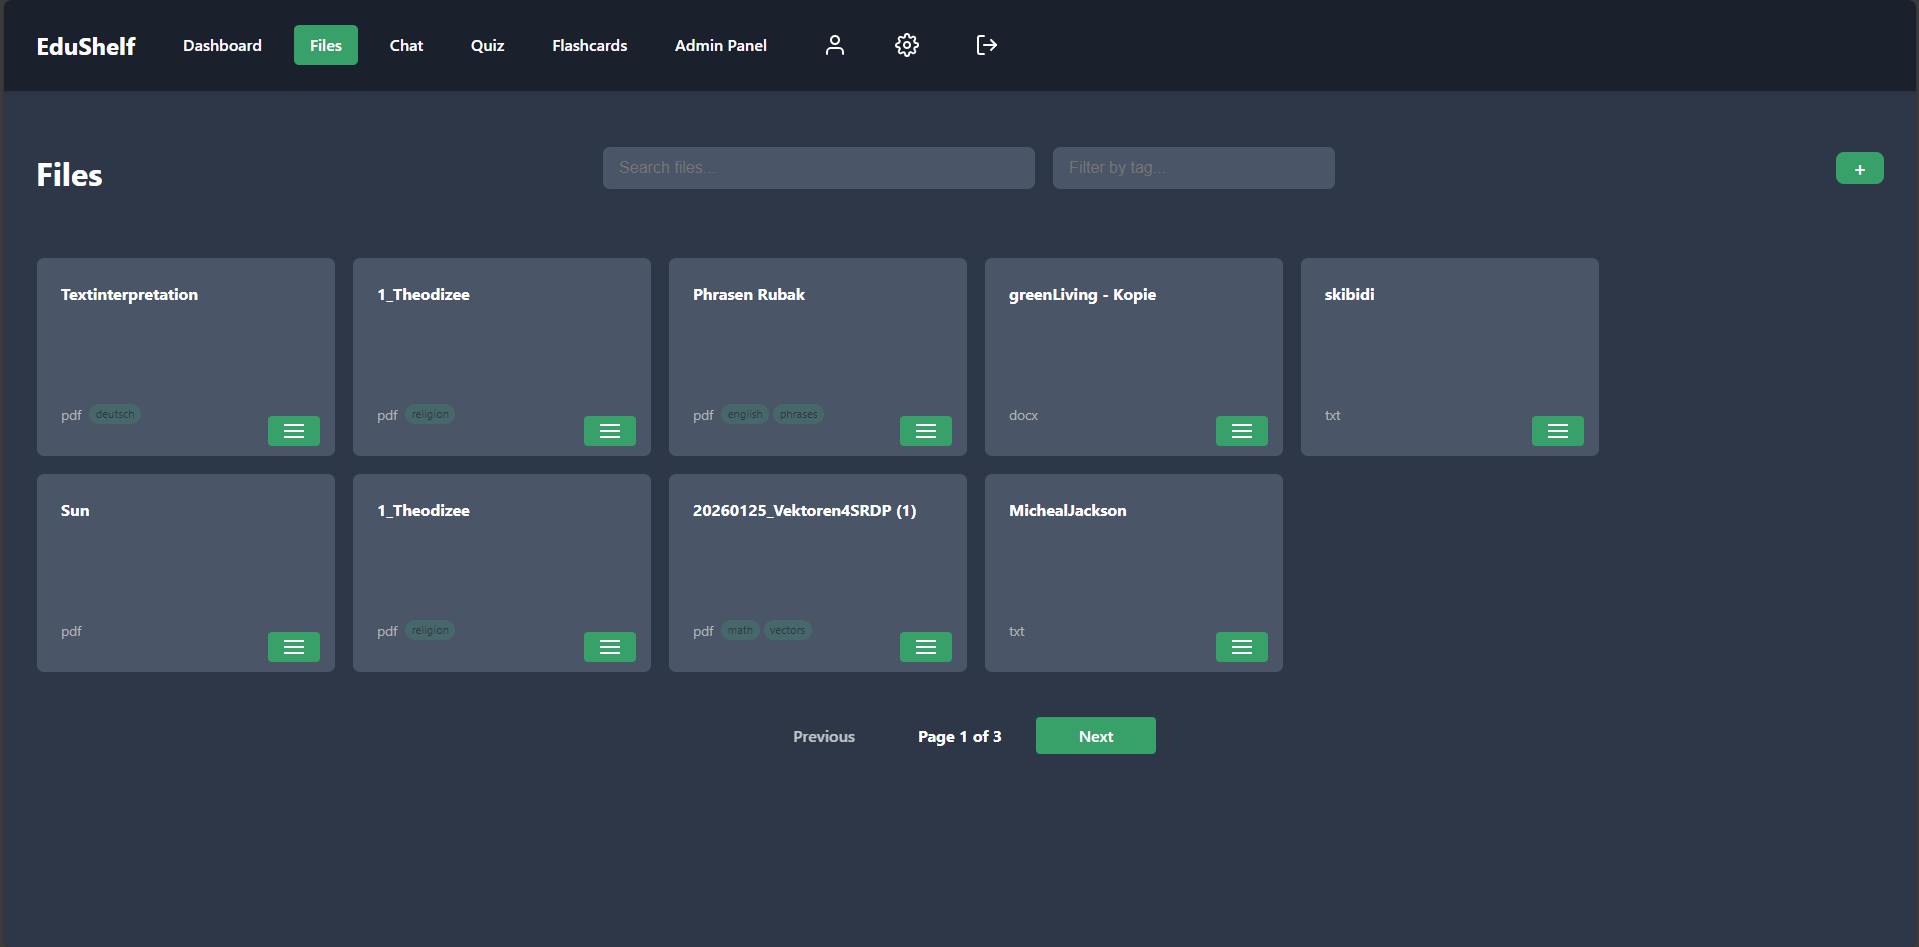
\includegraphics[width=0.92\textwidth]{img/files-dark-mode}
    \caption{Dateiübersicht von EduShelf im Dark-Mode}
    \label{fig:files}
\end{figure}


\subsection{Datenladen und Echtzeit-Suche}

Beim Laden der Komponente ruft ein \texttt{useEffect}-Hook die vollständige Dateiliste vom Server ab und speichert sie lokal im State. Die Suchfunktion operiert ausschließlich auf dieser lokalen Kopie -- es wird kein neuer API-Aufruf bei jeder Eingabe ausgelöst.

\begin{lstlisting}[language=JavaScript, caption={Clientseitige Echtzeit-Suche in der Dateiliste}]
const filteredFiles = files.filter(file =>
    file.name.toLowerCase().includes(searchTerm.toLowerCase())
);
\end{lstlisting}

Auch das Filtern erfolgt in Echtzeit über \texttt{Array.filter()}. Dieses Vorgehen ist sowohl performant als auch benutzerfreundlich: Da alle Daten bereits geladen sind, erfolgt das Filtern ohne wahrnehmbare Verzögerung, unabhängig von der Netzwerkqualität.


\subsection{Kontextmenü und Einzelaktionen}

Jede Datei in der Liste besitzt ein Kontextmenü, das über ein Drei-Punkte-Icon geöffnet wird. Der State \texttt{activeMenuId} speichert die ID der Datei, deren Menü aktuell geöffnet ist. Dadurch wird sichergestellt, dass immer nur ein Kontextmenü gleichzeitig sichtbar ist:

\begin{lstlisting}[language=JavaScript, caption={Menüsteuerung über activeMenuId}]
const toggleMenu = (fileId) => {
    setActiveMenuId(prev => (prev === fileId ? null : fileId));
};
\end{lstlisting}

Das Menü bietet folgende Optionen:
\begin{itemize}
    \item \textbf{Preview}: Öffnet die Vorschau mittels \texttt{FileViewer} direkt im Browser
    \item \textbf{Edit}: Ermöglicht das Bearbeiten von Tags
    \item \textbf{Share}: Öffnet das \texttt{ShareFileModal} zur Weitergabe an andere Nutzer
    \item \textbf{Delete}: Löscht die Datei und aktualisiert die Liste
    \item \textbf{Download}: Ermöglicht den Download von Files
\end{itemize}

\subsection{Upload-Prozess}

Der Dateiupload wird über ein Modal (\texttt{UploadDialog.jsx}) realisiert. Der Nutzer wählt eine Datei aus, die zusammen mit der User-ID als \texttt{multipart/form-data}~\cite{MDNFormData} an den Server gesendet wird. Nach erfolgreichem Upload wird \texttt{fetchFiles()} erneut aufgerufen, um die Ansicht ohne manuellen Seitenreload zu aktualisieren. Außerdem gibt es die Möglichkeit Tags hinzuzufügen, nach denen die Dateien später gefiltert werden können
\newpage

